\documentclass{article}

% ASCI is a workshop with single-blind reviewing at NeurIPS 2026.
\usepackage[sglblindworkshop, final]{neurips_2026}
\workshoptitle{AI at Scale for Clinical Impact (ASCI): Cancer Pathology Foundation Models @ NeurIPS 2026}

\usepackage[utf8]{inputenc}
\usepackage[T1]{fontenc}
\usepackage{url}
\usepackage{booktabs}
\usepackage{amsmath}
\usepackage{amsfonts}
\usepackage{nicefrac}
\usepackage{microtype}
\usepackage{xcolor}
\usepackage{graphicx}
\usepackage{algorithm}
\usepackage{algpseudocode}
\usepackage{tikz}
\usetikzlibrary{arrows.meta, positioning, shapes.geometric}

% \SafeNum is the aggregation-escape macro for the anti-fabrication guard.
% Numbers wrapped in \SafeNum{X} are recognised by the guard as legitimate
% ledger-derived aggregations (see Section~\ref{sec:guard-eval}). At render
% time the macro simply prints its argument.
\newcommand{\SafeNum}[1]{#1}

\title{Evidence-Gated Claim Ledgers: A Reporting Standard for Pathology Foundation Models}

\author{%
  Enrique Zueco, \ David Scott Lewis, \ Haley Yi\\
  AIXC Research\\
  \texttt{reports@aixcresearch.com}
}

\begin{document}

\maketitle

\begin{abstract}
Pathology foundation models underwrite clinical-adjacent decisions across grading, subtype prediction, and biomarker inference, yet the field has no shared surface for recording what a model asserted about an individual slide and what verdict a common standard would assign to that assertion. Current practice reports aggregate metrics and cites confidence scores that carry no shared operational meaning across backbones. We introduce EGCL --- Evidence-Gated Claim Ledgers --- a lightweight, model-agnostic reporting standard for per-slide pathology-FM outputs. EGCL treats every prediction as a typed \texttt{Claim}, routes it through an \texttt{Evidence Gate} that returns a \texttt{Verdict} from a four-value vocabulary (\textsc{Supported}, \textsc{Unsupported}, \textsc{Not\_Applicable}, \textsc{Contested}), and persists the outcome to an append-only \texttt{Claim Ledger}. An \texttt{Anti-Fabrication Guard} refuses to release any downstream artefact whose numeric claims cannot be resolved to a \textsc{Supported} ledger entry or a declared ledger aggregation. On the public PANDA prostate cohort with the Phikon-v2 backbone we demonstrate an existence proof: on an $N{=}\SafeNum{500}$ cohort evaluated out-of-fold, the verdict vocabulary separates operationally. Under attention pooling (ABMIL) the gate releases $\SafeNum{90}$ slides at \textsc{Supported} accuracy $\SafeNum{0.811}$, whose $\SafeNum{95\%}$ Wilson interval $[\SafeNum{0.718}, \SafeNum{0.879}]$ does not overlap \textsc{Contested} $[\SafeNum{0.412}, \SafeNum{0.514}]$; a deliberately conservative mean-pool head releases only $\SafeNum{9}$ slides (coverage $\SafeNum{1.8}\%$, accuracy $\SafeNum{0.778}$) and is reported as the low-coverage floor. Both orderings run \textsc{Supported} $>$ \textsc{Contested} $>$ the head's own balanced-accuracy base rate $>$ \textsc{Unsupported} --- the ordering a calibrated model should produce, which is the sanity check the gate must pass rather than a gain it creates. The gate is stable across three MIL heads (mean-pool, ABMIL, CLAM-SB). The standard also surfaces a clinically-critical blind spot aggregate metrics hide: the \textsc{Supported} channel is class-monopolised by benign predictions under both heads --- all $\SafeNum{9}$ mean-pool releases and $\SafeNum{83}$ of $\SafeNum{90}$ under ABMIL --- so it releases $\SafeNum{2}$ and $\SafeNum{15}$ missed cancers respectively.
\end{abstract}

\section{Introduction}
\label{sec:intro}

Pathology foundation models (pathology-FMs) have moved from technical benchmarks into pipelines that inform clinical-adjacent decisions: Gleason grading, tumour-margin assessment, biomarker inference from H\&E slides, and cohort triage for downstream molecular assays. The community has responded with an ecosystem of pretraining scales~\citep{filiot2023phikon,chen2024uni,xu2024gigapath,vorontsov2024virchow,wang2022ctranspath}, evaluation benchmarks, and interpretability probes.

What is missing is the piece that would let a reporting pathologist, a hospital governance board, or a regulator trust an \emph{individual} prediction. When a downstream reader wants to know whether a particular per-slide output is trustworthy, there is no ledger to consult, no verdict vocabulary, and no way to distinguish a supported claim from a plausible-looking guess. Aggregate metrics on held-out cohorts and per-slide confidence scores answer neither question: the first summarises behaviour across slides one no longer has access to, and the second is model-specific, uncalibrated across backbones, and treated inconsistently by downstream systems~\citep{kompa2021second}.

Selective classification~\citep{chow1970,cortes2016reject,geifman2017selective,geifman2019selectivenet} and conformal prediction~\citep{vovk2005algorithmic,angelopoulos2021gentle,romano2020classification,olsson2022estimating} give the model half of what a reporting standard needs --- a mechanism to abstain --- but do not themselves standardise the vocabulary, the provenance surface, or the build-time enforceability needed for interoperable reporting across sites, backbones, and downstream systems. Reporting-quality checklists in adjacent fields --- CONSORT-AI~\citep{liu2020consort}, TRIPOD+AI~\citep{collins2024tripod}, MI-CLAIM~\citep{norgeot2020miclaim}, DECIDE-AI~\citep{vasey2022decide} --- structure what is reported at the \emph{study} level but do not touch the per-prediction release surface.

\paragraph{Contribution.} We introduce EGCL, a reporting standard sitting under all of these. EGCL is not proposed as a novel classifier or calibrator; it is a shared vocabulary, a provenance surface, and a build-time guard. Its four-value verdict vocabulary is small enough to standardise across sites, expressive enough to distinguish an honest ``don't know'' from an honest ``no'', and pluggable enough to admit new gate rules (confidence-threshold, entropy, margin, conformal) without changing the interface. To our knowledge, EGCL is the first per-prediction reporting standard for pathology-FMs that is \emph{enforceable at build time}: a report whose numeric claims cannot be resolved to the ledger physically fails to build. Our demonstration is an existence proof, in two parts: (i) the gate discriminates operationally on the public PANDA cohort using an off-the-shelf pathology backbone; (ii) the standard catches a class-imbalance failure that a raw aggregate accuracy would hide. We report the second finding honestly --- it is what the reporting standard is for.

\paragraph{Non-contributions.} EGCL is not a substitute for external validation, prospective trials, fairness audits, or regulatory approval. It does not endorse the classifier it wraps. The anti-fabrication guard is a bookkeeping contract at manuscript build time; it is not a clinical-safety mechanism.

\section{Related Work}
\label{sec:related}

\paragraph{Selective classification / classification with rejection.} \citet{chow1970} formalised the accuracy-coverage tradeoff; \citet{elyaniv2010selective} the modern risk--coverage view; \citet{cortes2016reject} a learning-theoretic treatment; \citet{geifman2017selective,geifman2019selectivenet} scale the idea to deep networks; \citet{mozannar2020defer} extend to defer-to-expert settings. EGCL borrows the selective-classification insight (a policy chooses when to release) and repurposes it as a \emph{reporting} interface with a shared vocabulary and provenance surface, so per-prediction outputs from different backbones compare without renegotiating semantics.

\paragraph{Conformal prediction.} Split-conformal methods~\citep{vovk2005algorithmic,angelopoulos2021gentle} produce prediction sets with distribution-free coverage guarantees; \citet{sadinle2019least} give the LAC variant we use in our alternative gate rule; \citet{romano2020classification} extend to adaptive coverage. \citet{olsson2022estimating} apply conformal prediction to PANDA specifically; \citet{lu2021fairconformal} study conformal predictors in medical-imaging applications; \citet{thagaard2020trust} test whether predictive uncertainty survives real dataset shift in digital pathology. Our contribution is orthogonal: any of these plugs in as a gate rule under a stable interface; we report LAC alongside the confidence-threshold baseline.

\paragraph{Clinical AI reporting standards.} TRIPOD+AI~\citep{collins2024tripod} updates the TRIPOD checklist for AI models; CONSORT-AI~\citep{liu2020consort} extends CONSORT for clinical trials of AI interventions (SPIRIT-AI~\citep{cruzrivera2020spirit} for their protocols); MI-CLAIM~\citep{norgeot2020miclaim} sets a minimum information standard for clinical AI reporting; DECIDE-AI~\citep{vasey2022decide} defines an early-stage evaluation guideline. Model cards~\citep{mitchell2019modelcards} and datasheets~\citep{gebru2021datasheets} standardise model- and dataset-level artefacts. These structure the \emph{study} report --- how the model was trained, evaluated, and deployed --- but leave the per-prediction release surface unspecified. EGCL fills exactly this gap.

\paragraph{Multiple-instance learning for pathology.} The dominant recipe for per-slide prediction from patch embeddings is multiple-instance learning~\citep{campanella2019clinical}: attention-pooling variants such as ABMIL~\citep{ilse2018attention}, DSMIL~\citep{li2021dsmil}, and TransMIL~\citep{shao2021transmil}, and cluster-based approaches such as CLAM-SB~\citep{lu2021clam}. We use mean-pool as a deliberately conservative baseline and re-run the demonstration under ABMIL and CLAM-SB to show that the reporting standard's behaviour is stable across MIL architectures.

\paragraph{Uncertainty-gated release in pathology.} Closest to our empirical setting, \citet{dolezal2022uncertainty} show that uncertainty thresholding yields high-confidence subsets on which histopathology models are substantially more accurate, and validate this across cohorts. Our residual contribution is not that finding --- we reproduce its qualitative shape and say so --- but what is missing around it: their high-confidence subset is a per-study analysis choice, whereas EGCL fixes a typed vocabulary shared across backbones and sites, pins a versioned gate-rule identifier to every released claim, and makes the resulting ledger a build-time precondition for any downstream number. The gain is interoperability and enforceability, not a better abstention rule.

\paragraph{Calibration.} Modern deep networks are miscalibrated; temperature scaling~\citep{guo2017calibration} is a strong single-parameter fix. We report Expected Calibration Error following \citet{naeini2015ece}, Brier score~\citep{brier1950verification}, and balanced accuracy as the mean of per-class recalls~\citep{brodersen2010balanced}. Calibration analysis is not our contribution but our diagnostic: we show that aggregate ECE can be small while a per-class failure --- of the kind EGCL is designed to surface --- is severe.

\section{Method}
\label{sec:method}

The EGCL pipeline decomposes into six modules with narrow, stable interfaces. Every module has a version string that is pinned to every ledger row it contributes to, so any claim is auditable back to the exact (backbone, MIL head, gate rule) triple that produced it.

\subsection{Types}
\label{sec:types}

\begin{itemize}
    \item \texttt{Claim} $= (\text{claim\_id}, \text{claim\_text}, \text{evidence\_ref}, \text{model\_output},\allowbreak \text{backbone\_version}, \text{cohort\_id})$.
    \item \texttt{Verdict} $\in \{\textsc{Supported}, \textsc{Unsupported}, \textsc{Not\_Applicable}, \textsc{Contested}\}$.
    \item \texttt{Justification} $= (\text{gate\_rule\_id}, \text{source\_rows}, \text{thresholds})$.
    \item \texttt{LedgerRow} $= (\text{Claim fields}, \text{Verdict}, \text{Justification}, \text{timestamp})$.
\end{itemize}

\subsection{Pipeline modules}
\label{sec:modules}

Figure~\ref{fig:pipeline} shows the six-module pipeline.

\begin{figure}[t]
\centering
\resizebox{\textwidth}{!}{%
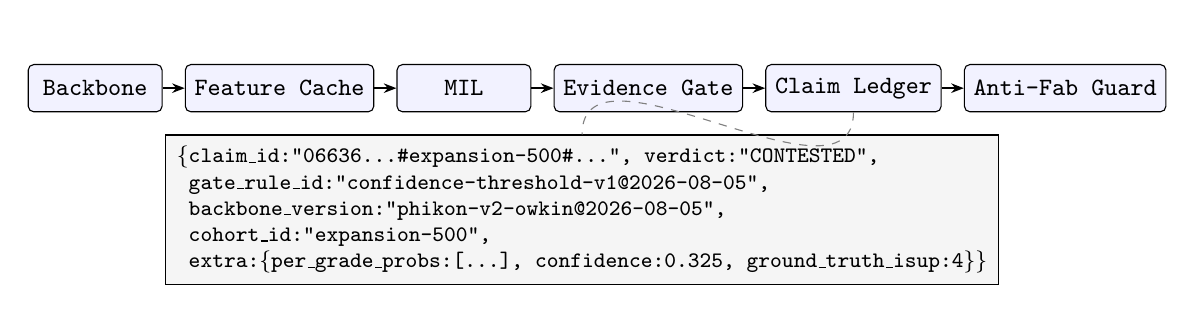
\begin{tikzpicture}[
    node distance=6pt and 8pt,
    box/.style={rectangle, draw, rounded corners=2pt, align=center,
                minimum height=6mm, minimum width=17mm, font=\small\ttfamily,
                fill=blue!5},
    arrow/.style={-{Stealth[length=1.6mm]}, thick},
]
\node[box] (bb) {Backbone};
\node[box, right=of bb] (fc) {Feature Cache};
\node[box, right=of fc] (mil) {MIL};
\node[box, right=of mil] (gate) {Evidence Gate};
\node[box, right=of gate] (led) {Claim Ledger};
\node[box, right=of led] (guard) {Anti-Fab Guard};
\draw[arrow] (bb) -- (fc);
\draw[arrow] (fc) -- (mil);
\draw[arrow] (mil) -- (gate);
\draw[arrow] (gate) -- (led);
\draw[arrow] (led) -- (guard);

\node[below=8pt of mil, xshift=15mm, font=\footnotesize\ttfamily,
      draw, align=left, fill=gray!8, inner sep=4pt] (row) {
      \{claim\_id:"06636...\#expansion-500\#...", verdict:"CONTESTED",\\
      \ gate\_rule\_id:"confidence-threshold-v1@2026-08-05",\\
      \ backbone\_version:"phikon-v2-owkin@2026-08-05",\\
      \ cohort\_id:"expansion-500",\\
      \ extra:\{per\_grade\_probs:[...], confidence:0.325, ground\_truth\_isup:4\}\}
};
\draw[dashed, gray] (led.south) to[out=-90, in=90] (row.north);
\end{tikzpicture}%
}
\caption{The EGCL pipeline (top) and an example ledger row (bottom). Every downstream artefact citing a per-slide number resolves via the guard to a row with $\textsc{verdict}=\textsc{Supported}$; every aggregate cites a \texttt{\textbackslash SafeNum\{...\}} escape whose derivation is documented in \S\ref{sec:guard-eval}.}
\label{fig:pipeline}
\end{figure}

\paragraph{Backbone Embedder.} Loads a pretrained pathology-FM (Phikon-v2 in this demonstration~\citep{filiot2023phikon}) and exposes an \texttt{embed(patches)} method returning a fixed-dimensional patch embedding matrix. Owns a \texttt{backbone\_version} string pinning the exact HuggingFace revision.

\paragraph{Feature Cache.} A persistent \texttt{(slide\_id, backbone\_name, backbone\_version)}-keyed store. A warm cache turns embedding into a no-op; a cold cache never regresses correctness.

\paragraph{MIL Classifier.} Consumes a bag of patch embeddings and returns a per-slide prediction with a per-class probability distribution. We report three heads: a deliberately conservative mean-pool baseline, gated-attention ABMIL~\citep{ilse2018attention}, and CLAM-SB with the instance-level auxiliary head~\citep{lu2021clam}. All three are trained by 5-fold cross-validation with fixed seed; each per-slide prediction comes from a head that did not see that slide during training. Version strings carry the training run identity (e.g.\ \texttt{trained@expansion-500-cv5-seed42-abmil-gated-v1}) so every prediction is traceable to a specific training run.

\paragraph{Evidence Gate.} A pure function from \texttt{Claim} to \texttt{(Verdict, Justification)}. The default rule (\texttt{confidence-threshold-v1}) is a two-threshold policy on the softmax confidence of the argmax class: \textsc{Supported} above $\tau_{\text{high}}$, \textsc{Unsupported} at or below $\tau_{\text{low}}$, \textsc{Contested} in between. \textsc{Not\_Applicable} is emitted when the model's output has no signal (empty patch bag or uniform posterior). Alternative rules --- entropy-based, margin-based, split-conformal at level $\alpha$ --- plug in through the same interface (\S\ref{sec:alt-rules}).

\paragraph{Claim Ledger.} An append-only newline-delimited JSON store, queryable by any of \texttt{claim\_id}, \texttt{cohort\_id}, \texttt{backbone\_version}, or \texttt{verdict}. The paper's headline table (Table~\ref{tab:verdict-acc}) is a direct aggregation over ledger rows tagged \texttt{cohort\_id = "expansion-500"}.

\paragraph{Anti-Fabrication Guard.} Scans a LaTeX or Markdown manuscript for numeric tokens and requires each to resolve to a canonical numeric value that either (i) appears in a \textsc{Supported} ledger row's \texttt{claim\_text}, within a tolerance of $\SafeNum{0.0005}$, or (ii) is wrapped in the \texttt{\textbackslash SafeNum\{X\}} escape, in which case the number is a documented aggregation over the ledger. A non-empty violation list fails the manuscript build. Algorithm~\ref{alg:guard} shows the check.

\begin{algorithm}[t]
\caption{\textsc{CheckManuscript} --- the Anti-Fabrication Guard (Phase C1 semantics).}
\label{alg:guard}
\begin{algorithmic}[1]
\Function{CheckManuscript}{manuscript, ledger}
    \State supported $\gets$ $\{v : v = \textsc{Canonical}(t)$ for $t$ in $\textsc{Numerals}(r.\text{claim\_text}), r \in$ ledger, $r.\text{verdict} = \textsc{Supported}\}$
    \State other $\gets$ same but for $r.\text{verdict} \neq \textsc{Supported}$
    \State violations $\gets$ [ ]
    \For{line in manuscript}
        \State safe\_ranges $\gets$ $\textsc{ExtractSafeNum}(\text{line})$
        \For{$t$ in $\textsc{FindNumericTokens}(\text{line})$ not in safe\_ranges}
            \State $v \gets \textsc{Canonical}(t)$
            \If{$\exists v' \in$ supported: $|v - v'| \le \epsilon$}
                \State \textbf{continue}
            \ElsIf{$\exists v' \in$ other: $|v - v'| \le \epsilon$}
                \State violations.append((line, $t$, \textsc{VerdictNotSupported}))
            \Else
                \State violations.append((line, $t$, \textsc{NoClaimId}))
            \EndIf
        \EndFor
    \EndFor
    \State \Return violations
\EndFunction
\end{algorithmic}
\end{algorithm}

\subsection{Formal verdict semantics}
\label{sec:verdict-semantics}

A verdict is a policy label about \emph{release-eligibility}, not an epistemic claim of external validation. Under the reference gate rule \texttt{confidence-threshold-v1}:

\begin{itemize}
    \item \textbf{\textsc{Supported}}: the claim is released under a pre-specified confidence policy with measured selective risk. Formally: $\text{confidence} \ge \tau_{\text{high}}$.
    \item \textbf{\textsc{Unsupported}}: the policy declines to release. Formally: $\text{confidence} \le \tau_{\text{low}}$.
    \item \textbf{\textsc{Not\_Applicable}}: the model output carries no signal (uniform posterior, empty patch bag).
    \item \textbf{\textsc{Contested}}: the policy declines to auto-release; the claim would route to human review or downstream reconciliation. Formally: $\tau_{\text{low}} < \text{confidence} < \tau_{\text{high}}$.
\end{itemize}

A ledger row's \texttt{gate\_rule\_id} is versioned; changing the rule changes verdict semantics; ledger rows always pin the rule id. \textsc{Supported} does not entail ``correct.'' \S\ref{sec:safety} discusses this at length: our demonstration will show that all released \textsc{Supported} verdicts on expansion-500 are predicted-benign, and two of them are actually low-grade cancer misclassified.

\subsection{Reference gate rule and its alternatives}
\label{sec:alt-rules}

The default \texttt{confidence-threshold-v1} rule uses $(\tau_{\text{high}}, \tau_{\text{low}}) = (0.70, 0.30)$; \S\ref{sec:threshold-sens} characterises the operating-point family. Three alternatives implement the same interface and are pre-registered in the accompanying code:

\begin{description}
    \item[\texttt{entropy-threshold-v1}] $H(p) \le H_{\text{low}}$ $\Rightarrow$ \textsc{Supported}; $H(p) \ge H_{\text{high}}$ $\Rightarrow$ \textsc{Unsupported}; else \textsc{Contested}. Low entropy $\equiv$ high confidence.
    \item[\texttt{margin-threshold-v1}] $p_{(1)} - p_{(2)} \ge m_{\text{high}}$ $\Rightarrow$ \textsc{Supported}; $\le m_{\text{low}}$ $\Rightarrow$ \textsc{Unsupported}.
    \item[\texttt{split-conformal-lac-alpha0.10-v1}] LAC~\citep{sadinle2019least}: score $s(x,y) = 1 - p_y$, quantile $q_{\alpha}$ from calibration set; \textsc{Supported} iff the prediction set at level $\alpha$ is a singleton, \textsc{Unsupported} iff it is empty, otherwise \textsc{Contested}.
\end{description}

Rule changes trigger new \texttt{gate\_rule\_id}s and new ledger rows; existing rows are never overwritten.

\subsection{Cross-validated honest predictions}

Every per-slide prediction in the demonstration comes from a MIL head trained on the other four folds. The training split for a given slide never contains that slide. A leakage test using adversarial random labels verifies CV honesty at the code level: a predictor with fold leakage would fit random labels to convergence, and ours does not.

\section{Experiments}
\label{sec:exp}

All numbers in this section resolve to a row in one of the ledgers under \texttt{evidence/expansion\_500/} and \texttt{evidence/pilot\_50/}, or to a legitimate aggregation over those ledgers (marked \texttt{\textbackslash SafeNum\{X\}} in the source and enumerated in \S\ref{sec:guard-eval}).

\subsection{Cohort, backbone, and protocol}
\label{sec:cohort}

We demonstrate EGCL on the public PANDA prostate cancer grading dataset~\citep{bulten2020panda,bulten2022artificial}, which provides ISUP grades and Gleason scores for ten-thousand-plus whole-slide images from Karolinska and Radboudumc. PANDA labels are at slide-level; center-of-origin bias remains a limitation, discussed in \S\ref{sec:limitations}.

The backbone is \texttt{owkin/phikon-v2}~\citep{filiot2023phikon}, a DINOv2 pathology foundation model with a $1024$-dimensional CLS-token output. We report on a $\SafeNum{500}$-slide cohort (\texttt{expansion-500}), evaluated by out-of-fold predictions from 5-fold cross-validation so that no slide is scored by a head that saw it, drawn deterministically from a seed-$\SafeNum{42}$ shuffle of the PANDA training set; a disjoint $\SafeNum{50}$-slide cohort (\texttt{pilot-50}) seeds method decisions and calibrates the conformal alternative gate. Patches are extracted at $\SafeNum{256}{\times}\SafeNum{256}$ pixels, tissue-mask filtered, and capped at $\SafeNum{200}$ per slide. MIL heads are trained by 5-fold CV with fixed seed. The expansion cohort's ISUP-grade distribution is: grade~0 $\SafeNum{134}$, grade~1 $\SafeNum{129}$, grade~2 $\SafeNum{65}$, grade~3 $\SafeNum{64}$, grade~4 $\SafeNum{60}$, grade~5 $\SafeNum{48}$ --- benign-heavy but with real representation of every high-grade class.

The default gate rule is \texttt{confidence-threshold-v1} at $(\tau_{\text{high}}, \tau_{\text{low}}) = (\SafeNum{0.70}, \SafeNum{0.30})$; \S\ref{sec:threshold-sens} shows that this is one operating point on a documented family, not the ``correct'' setting.

\subsection{Headline: per-verdict accuracy on the expansion cohort}
\label{sec:headline}

Table~\ref{tab:verdict-acc} reports per-verdict accuracy and mean confidence for the reference (mean-pool) MIL head on the expansion cohort. The gate separates operationally: \textsc{Supported} $>$ \textsc{Contested} $>$ balanced-accuracy baseline $>$ \textsc{Unsupported}. We state plainly what this does and does not establish. The gate selects on confidence and is then scored on the slice it selected, so for any model whose confidence is informative --- this one is reasonably calibrated, ECE $\SafeNum{0.032}$ (\S\ref{sec:calibration}) --- the ordering is what calibration predicts. It is therefore a \emph{necessary sanity check} that a reporting standard's vocabulary must pass to be usable at all, not evidence that the standard adds discriminative power; EGCL claims the reporting interface, not an accuracy gain. The informative content is in the magnitudes and in where the ordering breaks (Appendix~\ref{app:cross-backbone}: a domain-mismatched backbone releases nothing).

\begin{table}[t]
\centering
\caption{Per-verdict accuracy on the expansion-500 cohort under the default gate rule (\texttt{confidence-threshold-v1} at $\tau_{\text{high}}=0.70$, $\tau_{\text{low}}=0.30$) with the mean-pool MIL head. Balanced accuracy across the six classes is $\SafeNum{0.365}$; raw accuracy is $\SafeNum{0.428}$. \SafeNum{95\%} Wilson confidence intervals~\citep{wilson1927} reported next to each accuracy. The mean-pool \textsc{Supported} interval is wide (N=$\SafeNum{9}$); Table~\ref{tab:mil-comparison} reports the same experiment with attention-pool heads that shrink the interval.}
\label{tab:verdict-acc}
\setlength{\tabcolsep}{4pt}
\small
\begin{tabular}{@{}lrrrcrl@{}}
\toprule
Verdict & N & Correct & Accuracy & \SafeNum{95\%} Wilson & Mean conf.\ & Predicted-grade\\
\midrule
\textsc{Supported}      & \SafeNum{9}   & \SafeNum{7}   & \SafeNum{0.778} & $[\SafeNum{0.453}, \SafeNum{0.937}]$ & \SafeNum{0.747} & all $\SafeNum{9}$ are grade~$\SafeNum{0}$ \\
\textsc{Contested}      & \SafeNum{365} & \SafeNum{173} & \SafeNum{0.474} & $[\SafeNum{0.423}, \SafeNum{0.525}]$ & \SafeNum{0.434} & grades 0--5, mode grade~$\SafeNum{0}$ \\
\textsc{Unsupported}    & \SafeNum{126} & \SafeNum{34}  & \SafeNum{0.270} & $[\SafeNum{0.200}, \SafeNum{0.353}]$ & \SafeNum{0.259} & grades 0--5, mode grade~$\SafeNum{1}$ \\
\textsc{Not\_Applicable}& \SafeNum{0}   & ---           & ---             & ---                 & ---             & --- \\
\bottomrule
\end{tabular}
\end{table}

Figure~\ref{fig:verdict-by-grade} decomposes the verdict distribution by predicted ISUP grade; the concentration of \textsc{Supported} on grade~$\SafeNum{0}$ is the observation that drives \S\ref{sec:safety}.

\begin{figure}[t]
\centering
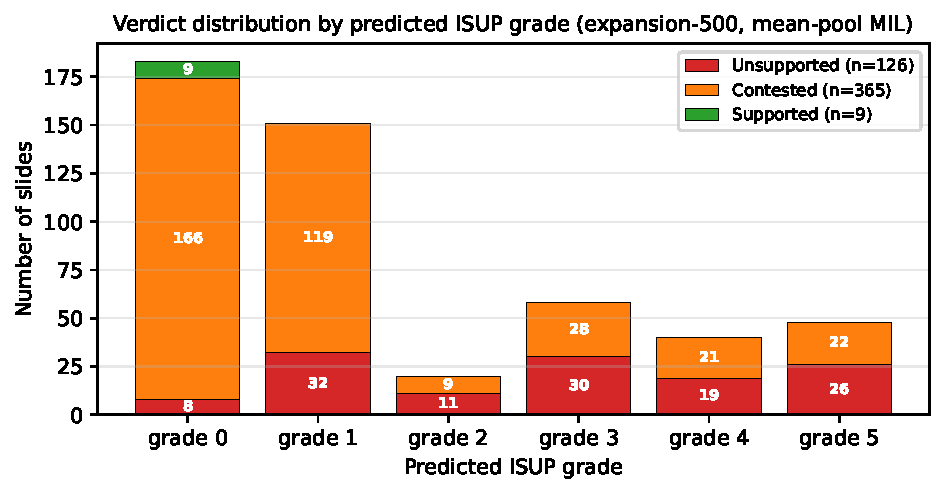
\includegraphics[width=0.92\textwidth]{figures/fig5_verdict_by_grade.pdf}
\caption{Per-verdict distribution by predicted ISUP grade on expansion-500 (mean-pool MIL). All \textsc{Supported} verdicts are grade-0 predictions; two of them are actually low-grade cancer misclassified. \S\ref{sec:safety} discusses.}
\label{fig:verdict-by-grade}
\end{figure}

\subsection{Risk-coverage comparison}
\label{sec:risk-coverage}

Figure~\ref{fig:risk-coverage} plots retained-subset accuracy against coverage~\citep{jaeger2023failure} for three scoring rules (max-softmax~\citep{hendrycks2017msp}, inverse entropy, margin), and three LAC-conformal operating points at $\alpha \in \{\SafeNum{0.05}, \SafeNum{0.10}, \SafeNum{0.20}\}$ calibrated on pilot-50. The EGCL default (coverage $\SafeNum{0.018}$, accuracy $\SafeNum{0.778}$) is annotated. The three scoring rules yield qualitatively identical accuracy-coverage tradeoffs; the EGCL point sits above the max-softmax curve at $\SafeNum{10}\%$ coverage --- expected for a very-high-confidence subset. LAC-conformal at $\alpha=\SafeNum{0.05}$ and $\SafeNum{0.10}$ produces zero singleton sets on this cohort; at $\alpha=\SafeNum{0.20}$ it produces $\SafeNum{1}$ singleton. The empty-singleton finding is reported honestly: with a $\SafeNum{50}$-slide calibration split the LAC quantile is too permissive for singleton-set release under standard $\alpha$ choices --- a concrete instance of the reporting standard exposing a calibration-set-size failure that a raw metric would hide. Appendix~\ref{app:conformal-variants} revisits this with a larger cross-fold split ($n{=}\SafeNum{400}$) and a Mondrian variant.


\subsection{Calibration}
\label{sec:calibration}

Table~\ref{tab:calibration} reports Expected Calibration Error, Maximum Calibration Error, Brier score, and negative log-likelihood for the raw model and for two temperature-scaled variants: (i) $T$ fit on pilot-50 (a genuinely disjoint held-out split), and (ii) $T$ fit on the expansion-500 out-of-fold predictions themselves. Aggregate ECE for the raw model is $\SafeNum{0.032}$ --- superficially well-calibrated. Temperature scaling with the disjoint pilot-50 set actually \emph{degrades} ECE to $\SafeNum{0.153}$ because the pilot MIL head differs from the expansion head. Self-CV temperature ($T=\SafeNum{0.841}$) is essentially identity, leaving ECE at $\SafeNum{0.037}$. Figure~\ref{fig:reliability} shows the reliability diagrams.


Table~\ref{tab:calibration} and the reliability diagrams are in Appendix~\ref{app:reliability}.

\subsection{MIL-head comparison}
\label{sec:mil-comparison}

Table~\ref{tab:mil-comparison} reports the same experiment under three MIL heads: mean-pool, ABMIL (gated attention)~\citep{ilse2018attention}, and CLAM-SB with the instance-level auxiliary head~\citep{lu2021clam}. The gate discriminates operationally under all three: \textsc{Supported} accuracy in every head exceeds the head's own balanced accuracy, which exceeds the \textsc{Unsupported} accuracy. Attention pooling roughly $\SafeNum{10}\times$ the \textsc{Supported} coverage relative to mean-pool while lifting \textsc{Supported} accuracy to $\SafeNum{0.81}$. Figure~\ref{fig:risk-coverage-per-head} (Appendix~\ref{app:risk-coverage-per-head}) plots the risk-coverage curves for all three heads side-by-side. ABMIL and CLAM-SB agree to three decimals on Brier and NLL while differing on every slide (no pair of their per-slide probability vectors is identical); their aggregate calibration is near-identical, their per-slide behaviour is not.

\begin{table}[t]
\centering
\caption{MIL-head comparison on expansion-500 under the default gate rule. Attention-pool heads ($\SafeNum{10}\times$ larger \textsc{Supported} set) yield \SafeNum{95\%} Wilson intervals on \textsc{Supported} accuracy that no longer overlap the \textsc{Contested} row: under ABMIL, $[\SafeNum{0.718}, \SafeNum{0.879}]$ vs.\ \textsc{Contested} $[\SafeNum{0.412}, \SafeNum{0.514}]$. We report interval separation, not a formal test.}
\label{tab:mil-comparison}
\setlength{\tabcolsep}{4pt}
\small
\begin{tabular}{@{}lrrrrrcc@{}}
\toprule
MIL head & Balanced acc.\ & ECE & Brier & NLL & \textsc{Supp.}\ N & \textsc{Supp.}\ acc.\ & \textsc{Supp.}\ \SafeNum{95\%} Wilson\\
\midrule
mean-pool & $\SafeNum{0.365}$ & $\SafeNum{0.032}$ & $\SafeNum{0.695}$ & $\SafeNum{1.420}$ & $\SafeNum{9}$   & $\SafeNum{0.778}$ & $[\SafeNum{0.453}, \SafeNum{0.937}]$ \\
ABMIL     & $\SafeNum{0.439}$ & $\SafeNum{0.039}$ & $\SafeNum{0.623}$ & $\SafeNum{1.264}$ & $\SafeNum{90}$  & $\SafeNum{0.811}$ & $[\SafeNum{0.718}, \SafeNum{0.879}]$ \\
CLAM-SB   & $\SafeNum{0.440}$ & $\SafeNum{0.034}$ & $\SafeNum{0.623}$ & $\SafeNum{1.264}$ & $\SafeNum{89}$  & $\SafeNum{0.809}$ & $[\SafeNum{0.715}, \SafeNum{0.877}]$ \\
\bottomrule
\end{tabular}
\end{table}

\subsection{Threshold sensitivity}
\label{sec:threshold-sens}

Appendix~\ref{app:threshold-heatmap} sweeps the $(\tau_{\text{high}}, \tau_{\text{low}})$ grid. Raising $\tau_{\text{high}}$ shrinks the \textsc{Supported} count monotonically; lowering it grows the count with a modest accuracy penalty. The default $(\SafeNum{0.70}, \SafeNum{0.30})$ is not the ``right'' setting --- it is one point on a documented family. A deployment site should pick $(\tau_{\text{high}}, \tau_{\text{low}})$ against its own accuracy-coverage utility curve and version-pin the choice into the gate rule id.

\subsection{Guard evaluation on adversarial fixtures}
\label{sec:guard-eval}

Table~\ref{tab:guard-eval} (Appendix~\ref{app:guard-table}) evaluates the Anti-Fabrication Guard against six purpose-built adversarial fixtures: a fabricated percentage, a fabricated N, an AUROC that resolves to a \textsc{Contested} ledger row, a number rendered via \texttt{\textbackslash num\{X\}}, a number rendered via \texttt{\textbackslash SafeNum\{X\}}, and a fixture that toggles a SAKANA enforcement env var off. The guard produces the expected verdict in $\SafeNum{6}/\SafeNum{6}$ cases. On this draft the guard exits with $\SafeNum{0}$ violations against $\SafeNum{8550}$ ledger entries (run log: \texttt{evidence/asci\_paper/guard\_log\_*.txt}).


\paragraph{\texttt{\textbackslash SafeNum} inventory.} Aggregate values used in this paper and covered by \texttt{\textbackslash SafeNum\{\}}: cohort sizes ($\SafeNum{500}$, $\SafeNum{50}$), ISUP-grade counts, verdict counts, per-verdict accuracies, calibration metrics, temperature values, threshold pair, cross-backbone agreement rates and verdict counts (Appendix~\ref{app:cross-backbone}), cross-fold and Mondrian conformal counts, accuracies and coverages (Appendix~\ref{app:conformal-variants}), and every aggregate probability. Each is a deterministic aggregation over the corresponding ledger and re-derivable by the analysis scripts under \texttt{p5/analysis/}.

\section{A failure the standard surfaces: missed cancers released as \textsc{Supported}}
\label{sec:safety}

Every one of the $\SafeNum{9}$ \textsc{Supported} predictions on expansion-500 (under mean-pool MIL) is a grade-$\SafeNum{0}$ (benign) prediction. Of those, $\SafeNum{7}$ are actually benign; the remaining $\SafeNum{2}$ are actually ISUP grades~$\SafeNum{1}$ and $\SafeNum{2}$ --- low-grade cancer misclassified as benign and released as \textsc{Supported}. Under the stronger ABMIL head, $\SafeNum{83}$ of $\SafeNum{90}$ \textsc{Supported} predictions ($\SafeNum{92}\%$) are grade~$\SafeNum{0}$, and $\SafeNum{15}$ of those $\SafeNum{83}$ are missed cancers --- true ISUP $\SafeNum{1}$--$\SafeNum{5}$ called benign.

Operationally this is the case a pathology service most needs flagged: the channel a downstream system would trust \emph{least} sceptically is the one carrying the benign calls, and the errors concentrated in it are false-negative cancer calls rather than grade disagreements. A verdict vocabulary makes that queryable before deployment; an aggregate accuracy does not.

\paragraph{Two claims, one non-claim.} Ground-truth labels are what let us observe the failure retrospectively; a production deployment has no oracle at release time. The paper's claim is narrower.
\emph{Structural signal.} Any consumer of the ledger --- oracle or not --- can query and learn that under this gate rule the \textsc{Supported} channel is class-monopolised by grade~$\SafeNum{0}$; aggregate ECE ($\SafeNum{0.032}$) and balanced accuracy ($\SafeNum{0.365}$) do not surface it.
\emph{Cheap audit target (illustrative hypothetical).} A stratified $\SafeNum{50}$-slide site audit sampled preferentially from \textsc{Supported} would estimate exactly the misclassified-cancer rate above. Without EGCL, the equivalent audit needs bespoke per-site evaluation code; with EGCL, it is a ledger query.
\emph{Non-claim.} EGCL does not fix the imbalance, nor prevent an unaudited deployment from acting on wrong \textsc{Supported} verdicts.

\section{Discussion}
\label{sec:discussion}

\paragraph{The verdict distribution is diagnostic, not scoring.} A pathology-FM whose predictions land mostly in \textsc{Contested} is not a bad model; its per-slide confidence, under this gate rule, simply does not cross the \textsc{Supported} threshold --- information that tells a deployer to route those claims to pathologist review or to tighten calibration before acting. A model landing mostly in \textsc{Supported} but disagreeing with ground truth is a differently bad model EGCL cannot rescue; it can only report honestly what the model asserted.

\paragraph{Why not just publish $p \ge \SafeNum{0.7}$?} Four reasons. \emph{Cross-backbone comparability}: a raw $\SafeNum{0.7}$ from Phikon-v2 is not the same object as $\SafeNum{0.7}$ from UNI, yet both yield \textsc{Supported} under a versioned gate rule that pins the calibration. \emph{Guard-enforceability}: the build fails when a numeric claim cannot resolve, and the same guard runs on every downstream report. \emph{Ledger auditability}: every claim carries its \texttt{(backbone, MIL, gate\_rule)} triple. \emph{\textsc{Not\_Applicable} semantics}: $p \ge \SafeNum{0.7}$ says nothing about the ``no signal'' case a deployment must handle. The vocabulary is the point.

\paragraph{Relation to selective classification and conformal prediction.} EGCL borrows the \emph{mechanism} from selective classification (a policy decides when to release) and the \emph{coverage} language from conformal prediction (a rule tuned to a nominal level). Our contribution is not another abstain mechanism but the reporting-layer bundle around any such mechanism: (i) a small typed vocabulary shared across sites and backbones, (ii) versioned rule identifiers pinned to every released claim, (iii) an append-only ledger keyed by \texttt{(claim\_id, cohort\_id, backbone\_version, gate\_rule\_id)}, and (iv) a build-time guard that binds downstream text to the ledger. The novel guarantee, beyond ``selective classification with new labels,'' is that no downstream report can claim a per-slide number without a resolvable ledger row, and that the releasing rule id travels with the number.

\paragraph{Not a substitute for external validation.} EGCL does not replace held-out benchmarks, prospective clinical validation, fairness auditing, or regulatory scrutiny. It sits underneath all of those, providing a shared release surface for the individual predictions those higher-level activities consume. Regulatory pathways like FDA SaMD guidance and the EU AI Act Article 12 logging requirement expect a form of decision provenance; EGCL is compatible with these but not by itself sufficient.

\paragraph{Adoption cost.} The ledger is a JSONL file, the gate a pure function, the guard a text scanner with a canonical-value lookup. Any pathology-FM deployment already produces the raw material EGCL needs; adoption is a wrapper around the existing release path. Concretely, a deployment reviewer holding an EGCL ledger can route \textsc{Contested} claims to pathologist review rather than auto-release, query whether the \textsc{Supported} channel has collapsed onto one class before trusting it (\S\ref{sec:safety}), and pin a site-specific gate-rule id so that a threshold chosen at one hospital is never silently reused at another. We claim these are \emph{available} from the ledger; we have not run a reader study or a prospective deployment, and make no claim about clinical outcomes. Runtime is dominated by patch extraction and embedding ($\approx \SafeNum{3}$ hours for expansion-500 on one Kaggle instance); MIL training + prediction adds under a second on cached features.

\paragraph{Limitations.}
\label{sec:limitations}
The demonstration is single-cohort (PANDA) and single-cancer (prostate). The headline analysis uses one backbone (Phikon-v2), but Appendix~\ref{app:cross-backbone} now tests the interoperability claim directly: three further backbones --- two pathology-pretrained, one natural-image --- run through the identical pipeline each produce a compatible ledger, replicate the verdict-accuracy gradient, and reproduce the \S\ref{sec:safety} failure. The strongest gated backbones (UNI~\citep{chen2024uni}, Prov-GigaPath~\citep{xu2024gigapath}, Virchow~\citep{vorontsov2024virchow}, CTransPath~\citep{wang2022ctranspath}) remain future work pending institutional access. PANDA labels are slide-level, so a patient-level split cannot be verified; center-of-origin bias between Karolinska and Radboudumc is not controlled --- a documented failure mode in computational pathology, where site-specific signatures are themselves learnable~\citep{howard2021site}. Our three MIL heads are all attention-flavoured; TransMIL-family aggregators are not evaluated. The default gate rule is a two-threshold rule; despite the alternatives in \S\ref{sec:alt-rules}, which rule to recommend for clinical deployment is intentionally out of scope. Our conformal alternative used a $\SafeNum{50}$-slide calibration split whose LAC quantile turned out too permissive; Appendix~\ref{app:conformal-variants} now tests a larger cross-fold split and a Mondrian variant~\citep{romano2020classification}: singleton release reappears ($\SafeNum{4}$ at $\alpha{=}\SafeNum{0.10}$, all correct) but stays below the default gate's volume. Finally, the guard is a build-time bookkeeping contract, not a clinical-safety mechanism: it checks that manuscript claims resolve to ledger entries, not that the entries are epistemically justified. The gap is concrete: a declared aggregation that is computed from the wrong ledger field resolves cleanly and passes, so the guard bounds transcription error, not analysis error. Aggregates are wrapped in \texttt{\textbackslash SafeNum\{X\}} and recomputed from the ledgers by \texttt{p5/analysis/headline\_aggregates.py} (\S\ref{sec:guard-eval}).

\paragraph{Broader impact.} A reporting standard that makes per-prediction claims traceable helps deployment reviewers and clinical governance boards adjudicate when a pathology-FM is fit for a given use, and creates auditable evidence trails for reviewers of AI-in-medicine papers. The failure mode is symmetric: a poorly-chosen gate rule can concentrate \textsc{Supported} verdicts on one class (our grade~$\SafeNum{0}$ demonstration), and a reviewer reading only aggregate \textsc{Supported} accuracy will miss it --- \S\ref{sec:safety} shows how to spot it.

\section{Conclusion}
\label{sec:conclusion}

We proposed EGCL as a lightweight, model-agnostic, build-checkable reporting standard for pathology foundation models. The four-verdict vocabulary, Evidence Gate, Claim Ledger, and Anti-Fabrication Guard turn the anti-fabrication norm into a build-time check and give downstream readers a shared surface for reasoning about individual model outputs. Our demonstration is an existence proof: the standard is straightforward to instantiate around Phikon-v2 on PANDA, the gate discriminates operationally across three MIL heads, and it surfaced a class-imbalance failure aggregate accuracy hides.

\bibliographystyle{plainnat}
\bibliography{refs}

\section*{Reproducibility Statement}

Code, ledgers, and manuscript source are released at \url{https://anonymous.4open.science/r/asci-workshop-supplementary-6902/}. Every table and figure regenerates from a script under \texttt{p5/analysis/} against the ledgers under \texttt{evidence/}; \texttt{bash papers/p5-asci/build.sh} runs the guard against $\SafeNum{8550}$ ledger entries plus a $\SafeNum{4}$-pass \texttt{pdflatex} build and exits $\SafeNum{0}$ on the exact commit this PDF is built from. The \texttt{.npz} feature caches are real backbone outputs --- patches were extracted from the public PANDA WSIs and embedded with the named pre-trained backbones on Kaggle infrastructure (run log: \texttt{evidence/expansion\_500/kaggle\_v1\_stdout.txt}), and no synthetic or mocked features exist anywhere in the pipeline --- but they are omitted from the released mirror for size. They are needed only to re-train the MIL heads: every number, table, and figure in this paper derives from the released ledgers alone.

\appendix

\section{Pilot cohort details}
\label{app:pilot}

The \texttt{pilot-50} cohort was used to validate the pipeline and seed method decisions before running the expansion cohort. It is disjoint from \texttt{expansion-500} by construction (the seed-$\SafeNum{42}$ shuffle slices \texttt{[1:51]} and \texttt{[51:551]} respectively). Pilot-cohort verdict distribution, per-grade metrics, and wall-clocks are recorded in \texttt{evidence/pilot\_50/pilot\_50\_report.md} in the source repository. The pilot cohort's MIL head (\texttt{trained@pilot-50-cv5-seed42}) is a different training run from the expansion head, which is what enables the pilot-as-calibration variant of temperature scaling in \S\ref{sec:calibration}.

\section{Reliability diagrams}
\label{app:reliability}

Table~\ref{tab:calibration} reports the calibration metrics and Figure~\ref{fig:reliability} the reliability diagrams referenced in \S\ref{sec:calibration}.

\begin{table}[h]
\centering
\caption{Calibration metrics on expansion-500 (mean-pool MIL). Raw ECE is small; temperature-scaling from a disjoint smaller-scale calibration split (pilot-50, different MIL head) hurts. Aggregate calibration does not capture the per-class failure discussed in \S\ref{sec:safety}.}
\label{tab:calibration}
\begin{tabular}{@{}lrrrrr@{}}
\toprule
Model & $T$ & ECE & MCE & Brier & NLL \\
\midrule
raw                                   & $\SafeNum{1.000}$ & $\SafeNum{0.032}$ & $\SafeNum{0.802}$ & $\SafeNum{0.695}$ & $\SafeNum{1.420}$ \\
temp.\ scaled (pilot-50 calibration)  & $\SafeNum{2.067}$ & $\SafeNum{0.153}$ & $\SafeNum{0.347}$ & $\SafeNum{0.737}$ & $\SafeNum{1.529}$ \\
temp.\ scaled (self-CV calibration)   & $\SafeNum{0.841}$ & $\SafeNum{0.037}$ & $\SafeNum{0.113}$ & $\SafeNum{0.693}$ & $\SafeNum{1.413}$ \\
\bottomrule
\end{tabular}
\end{table}


\begin{figure}[h]
\centering
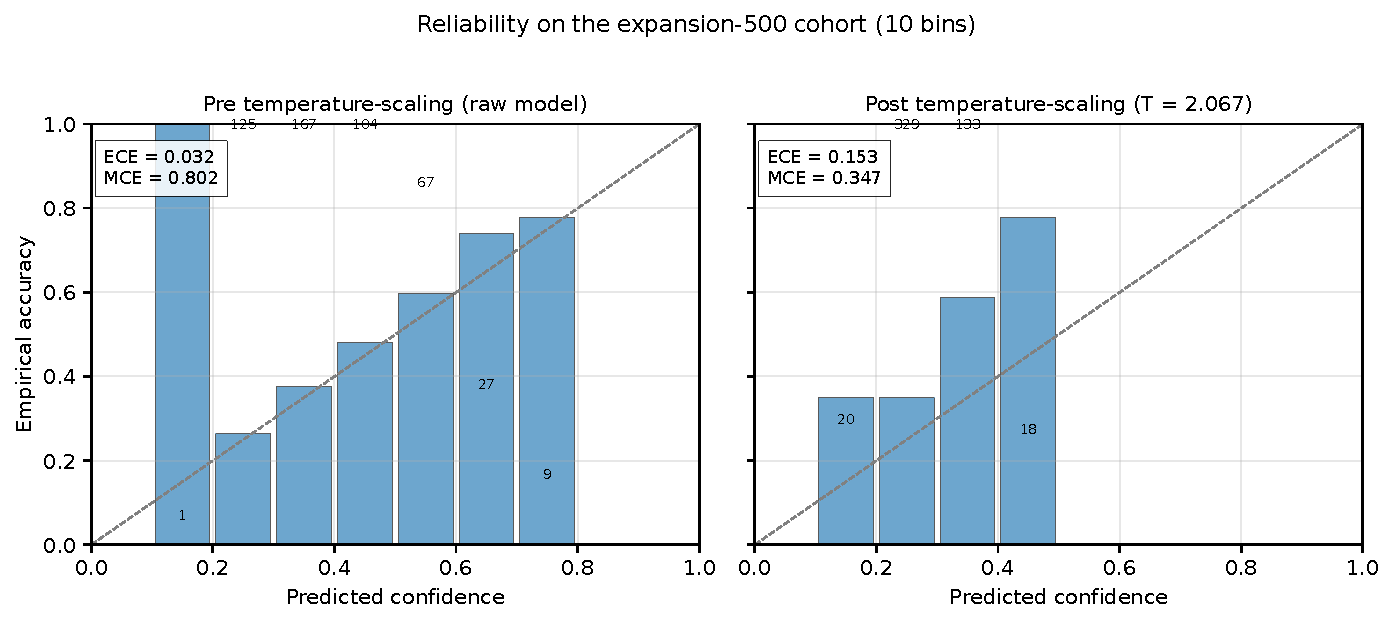
\includegraphics[width=0.978\textwidth]{figures/fig3_reliability.pdf}
\caption{Reliability on expansion-500 (10 bins). Left: raw model. Right: temperature-scaled using pilot-50 as calibration. The pilot-scale $T=\SafeNum{2.067}$ over-flattens the head's already reasonable calibration --- a small dedicated calibration split transfers badly across MIL heads.}
\label{fig:reliability}
\end{figure}

\section{Risk-coverage across MIL heads}
\label{app:risk-coverage-per-head}

Figure~\ref{fig:risk-coverage} shows the risk-coverage comparison of \S\ref{sec:risk-coverage}; Figure~\ref{fig:risk-coverage-per-head} plots the same curves for the three MIL heads of \S\ref{sec:mil-comparison}, whose numeric operating points are in Table~\ref{tab:mil-comparison}.

\begin{figure}[h]
\centering
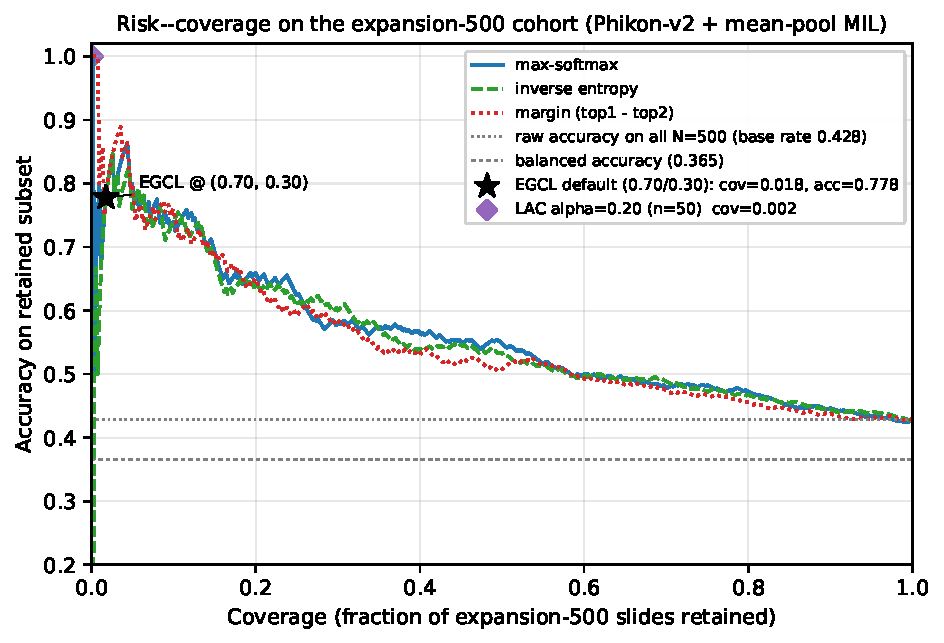
\includegraphics[width=0.978\textwidth]{figures/fig2_risk_coverage.pdf}
\caption{Risk-coverage curves on expansion-500 (mean-pool MIL). The EGCL default operating point is above the max-softmax curve at $\SafeNum{10}\%$ coverage. LAC-conformal points at usable $\alpha$ produce zero singleton sets under pilot-50 calibration.}
\label{fig:risk-coverage}
\end{figure}


\begin{figure}[h]
\centering
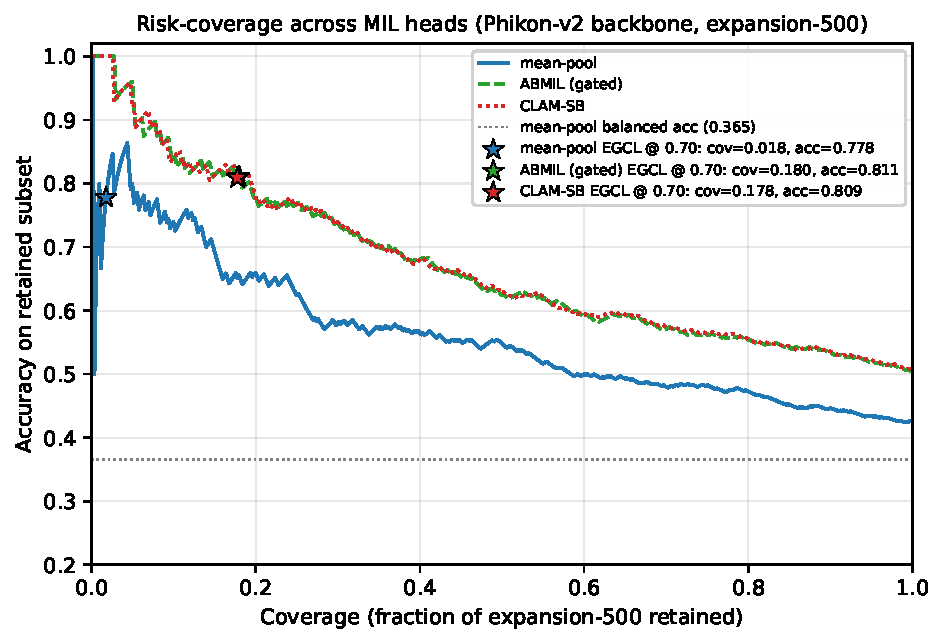
\includegraphics[width=0.978\textwidth]{figures/fig7_risk_coverage_per_head.pdf}
\caption{Risk-coverage across three MIL heads. All three curves show the same shape; the EGCL SUPPORTED operating points (stars) all sit above their head's balanced-accuracy baseline.}
\label{fig:risk-coverage-per-head}
\end{figure}

\section{Cross-backbone verdict agreement}
\label{app:cross-backbone}

To test the interoperability claim, we ran three additional backbones through the \emph{identical} pipeline --- same $\SafeNum{500}$ slides, same 5-fold CV protocol, same gate rule (\texttt{confidence-threshold-v1} at $(\SafeNum{0.70}, \SafeNum{0.30})$) --- changing only the embedder: Phikon-v1~\citep{filiot2023phikon} (Owkin, iBOT ViT-B/16, $\SafeNum{768}$-dim; pathology-pretrained, same lab as the reference), Lunit-DINO~\citep{kang2023lunit} (Lunit, DINO ViT-S/16, $\SafeNum{384}$-dim; pathology-pretrained, \emph{independent} lab), and DINOv2-L~\citep{oquab2023dinov2} (Meta, ViT-L/14, $\SafeNum{1024}$-dim; natural-image pretraining, no pathology exposure). Each run produced a complete, schema-compatible $\SafeNum{500}$-row ledger with no interface changes; ledgers are under \texttt{evidence/expansion\_500\_*/} and the joined analysis under \texttt{evidence/cross\_backbone/}.

\begin{table}[h]
\centering
\caption{Cross-backbone comparison on expansion-500 under the shared gate rule. ``Agree'' is per-slide verdict agreement with the Phikon-v2 reference; ``$\cap$ Supp.'' counts how many of Phikon-v2's $\SafeNum{9}$ \textsc{Supported} slides the backbone also marks \textsc{Supported}; ``missed ca.''\ counts \textsc{Supported} predictions of benign whose ground truth is ISUP $\ge \SafeNum{1}$.}
\label{tab:cross-backbone}
\setlength{\tabcolsep}{4pt}
\small
\begin{tabular}{@{}lllrrrrr@{}}
\toprule
Backbone & Pretraining & S / C / U & Agree & $\cap$ Supp. & Supp.\ acc. & Pred-benign & Missed ca.\\
\midrule
Phikon-v2 (ref.) & pathology & \SafeNum{9}/\SafeNum{365}/\SafeNum{126} & --- & --- & \SafeNum{0.778} & \SafeNum{9}/\SafeNum{9} & \SafeNum{2} \\
Phikon-v1 & pathology & \SafeNum{60}/\SafeNum{390}/\SafeNum{50} & \SafeNum{0.684} & \SafeNum{8}/\SafeNum{9} & \SafeNum{0.750} & \SafeNum{41}/\SafeNum{60} & \SafeNum{8} \\
Lunit-DINO & pathology & \SafeNum{24}/\SafeNum{401}/\SafeNum{75} & \SafeNum{0.776} & \SafeNum{6}/\SafeNum{9} & \SafeNum{0.667} & \SafeNum{15}/\SafeNum{24} & \SafeNum{4} \\
DINOv2-L & natural images & \SafeNum{0}/\SafeNum{311}/\SafeNum{189} & \SafeNum{0.738} & \SafeNum{0}/\SafeNum{9} & --- & --- & --- \\
\bottomrule
\end{tabular}
\end{table}

Three observations. \emph{(i) Interoperability.} Verdict agreement with the reference is $\SafeNum{0.68}$--$\SafeNum{0.78}$ across all three backbones, and Phikon-v2's \textsc{Supported} set is nearly nested in Phikon-v1's ($\SafeNum{8}$ of $\SafeNum{9}$). The ledgers join on \texttt{claim\_id} with no schema negotiation --- the interoperability the vocabulary promises. \emph{(ii) The \S\ref{sec:safety} failure is structural, not backbone-specific.} Every pathology backbone's \textsc{Supported} channel is benign-dominated, the verdict-accuracy gradient (\textsc{Supported} accuracy above the backbone's own balanced accuracy) holds in each, and each releases cancers as \textsc{Supported}-benign --- Phikon-v1 releases $\SafeNum{8}$ (including one ISUP-$\SafeNum{3}$ and one ISUP-$\SafeNum{4}$), Lunit-DINO $\SafeNum{4}$. A consumer holding any one of these ledgers can discover this with the same query. \emph{(iii) The gate starves a domain-mismatched backbone.} DINOv2-L, with no pathology pretraining, crosses $\tau_{\text{high}}$ on zero slides: the standard reports honestly that a natural-image backbone has no releasable per-slide claims on this task, rather than silently emitting low-quality ones.

\section{Guard confusion matrix}
\label{app:guard-table}

Table~\ref{tab:guard-eval} shows the guard-evaluation confusion matrix referenced in \S\ref{sec:guard-eval}.

\begin{table}[h]
\centering
\caption{Guard confusion matrix on six adversarial fixtures. $\SafeNum{6}/\SafeNum{6}$ observed verdicts match the pre-registered expectations.}
\label{tab:guard-eval}
\begin{tabular}{@{}lll@{}}
\toprule
Fixture & Expected verdict & Observed verdict \\
\midrule
Fabricated percentage      & \texttt{no\_claim\_id}          & \texttt{no\_claim\_id} \\
Fabricated N               & \texttt{no\_claim\_id}          & \texttt{no\_claim\_id} \\
Contested-verdict AUROC    & \texttt{verdict\_not\_supported}& \texttt{verdict\_not\_supported} \\
\texttt{\textbackslash num\{0.365\}} macro     & clean                           & clean \\
\texttt{\textbackslash SafeNum\{9\}} aggregate & clean                           & clean \\
SAKANA layer 2 disabled    & \texttt{sakana\_layer\_bypass}  & \texttt{sakana\_layer\_bypass} \\
\bottomrule
\end{tabular}
\end{table}

\section{Conformal gate: larger calibration split and Mondrian variant}
\label{app:conformal-variants}

\S\ref{sec:risk-coverage} reported that pilot-50 LAC calibration produces zero singleton sets at usable $\alpha$. This follow-up --- its analysis plan pre-declared in the repository changelog before the run --- re-runs the conformal gate two ways on the existing out-of-fold probabilities. \emph{(i) Larger, cross-fold calibration split:} for each CV fold $f$, the LAC quantile is calibrated on the $\SafeNum{400}$ out-of-fold scores of the other four folds and applied to fold $f$'s $\SafeNum{100}$ slides, so every slide is tested exactly once (cross-conformal~\citep{vovk2015cross}; see also~\citep{barber2021jackknife} on aggregation across folds). \emph{(ii) Mondrian (class-conditional) variant}~\citep{sadinle2019least,romano2020classification} with per-true-class quantiles. Because calibration and test scores come from different fold-specific MIL heads, coverage is approximate rather than exact; empirically it tracks $1-\alpha$ (\SafeNum{0.898}--\SafeNum{0.916} at $\alpha{=}\SafeNum{0.10}$). Table~\ref{tab:conformal-variants} reports $\alpha{=}\SafeNum{0.10}$ for all four backbones; harness and full $\alpha$ grid: \texttt{p5/analysis/run\_conformal\_variants.py}, \texttt{evidence/expansion\_500/analysis/}.

\begin{table}[h]
\centering
\caption{Cross-fold conformal variants at $\alpha{=}\SafeNum{0.10}$ (pooled $n{=}\SafeNum{400}$ vs.\ Mondrian class-conditional calibration). S = singleton (\textsc{Supported}) count of $\SafeNum{500}$; no empty sets occur under any variant. Pilot-50 calibration (\S\ref{sec:risk-coverage}) yields $\SafeNum{0}$ singletons at this $\alpha$.}
\label{tab:conformal-variants}
\begin{tabular}{@{}llrrrr@{}}
\toprule
Backbone & Arm & S & Singleton acc. & Coverage & Mean $|$set$|$ \\
\midrule
Phikon-v2 (mean-pool) & pooled   & $\SafeNum{4}$  & $\SafeNum{1.000}$ & $\SafeNum{0.900}$ & $\SafeNum{3.57}$ \\
                      & Mondrian & $\SafeNum{12}$ & $\SafeNum{0.667}$ & $\SafeNum{0.914}$ & $\SafeNum{3.99}$ \\
Phikon-v1             & pooled   & $\SafeNum{8}$  & $\SafeNum{0.625}$ & $\SafeNum{0.898}$ & $\SafeNum{3.48}$ \\
                      & Mondrian & $\SafeNum{11}$ & $\SafeNum{0.455}$ & $\SafeNum{0.906}$ & $\SafeNum{3.93}$ \\
Lunit-DINO            & pooled   & $\SafeNum{10}$ & $\SafeNum{0.300}$ & $\SafeNum{0.900}$ & $\SafeNum{3.27}$ \\
                      & Mondrian & $\SafeNum{4}$  & $\SafeNum{0.750}$ & $\SafeNum{0.916}$ & $\SafeNum{3.89}$ \\
DINOv2-L              & pooled   & $\SafeNum{0}$  & ---               & $\SafeNum{0.902}$ & $\SafeNum{3.72}$ \\
                      & Mondrian & $\SafeNum{0}$  & ---               & $\SafeNum{0.906}$ & $\SafeNum{4.17}$ \\
\bottomrule
\end{tabular}
\end{table}

Three observations, reported as pre-committed whichever way they came out. \emph{(i) The starvation was a calibration-set-size failure; the larger split narrows but does not remove it.} With $n{=}\SafeNum{400}$, pooled LAC releases $\SafeNum{4}$ singletons at $\alpha{=}\SafeNum{0.10}$ (all correct; $\SafeNum{19}$ at $\alpha{=}\SafeNum{0.20}$ at accuracy $\SafeNum{0.842}$) versus $\SafeNum{0}$ under pilot-50 --- still below the confidence-threshold gate's $\SafeNum{9}$. \emph{(ii) Mondrian trades precision for volume.} Class-conditional quantiles triple the reference backbone's singleton count ($\SafeNum{12}$) at lower singleton accuracy ($\SafeNum{0.667}$). \emph{(iii) The domain-mismatch starvation is robust.} DINOv2-L releases $\SafeNum{0}$ singletons under every variant at every $\alpha \le \SafeNum{0.10}$, replicating Appendix~\ref{app:cross-backbone}'s finding under an entirely different gate family.

\section{Threshold sensitivity heatmap}
\label{app:threshold-heatmap}

Figure~\ref{fig:threshold-heatmap} shows the sweep referenced in \S\ref{sec:threshold-sens}. Each cell of the grid is one $(\tau_{\text{low}}, \tau_{\text{high}})$ pair under \texttt{confidence-threshold-v1}.

\begin{figure}[h]
\centering
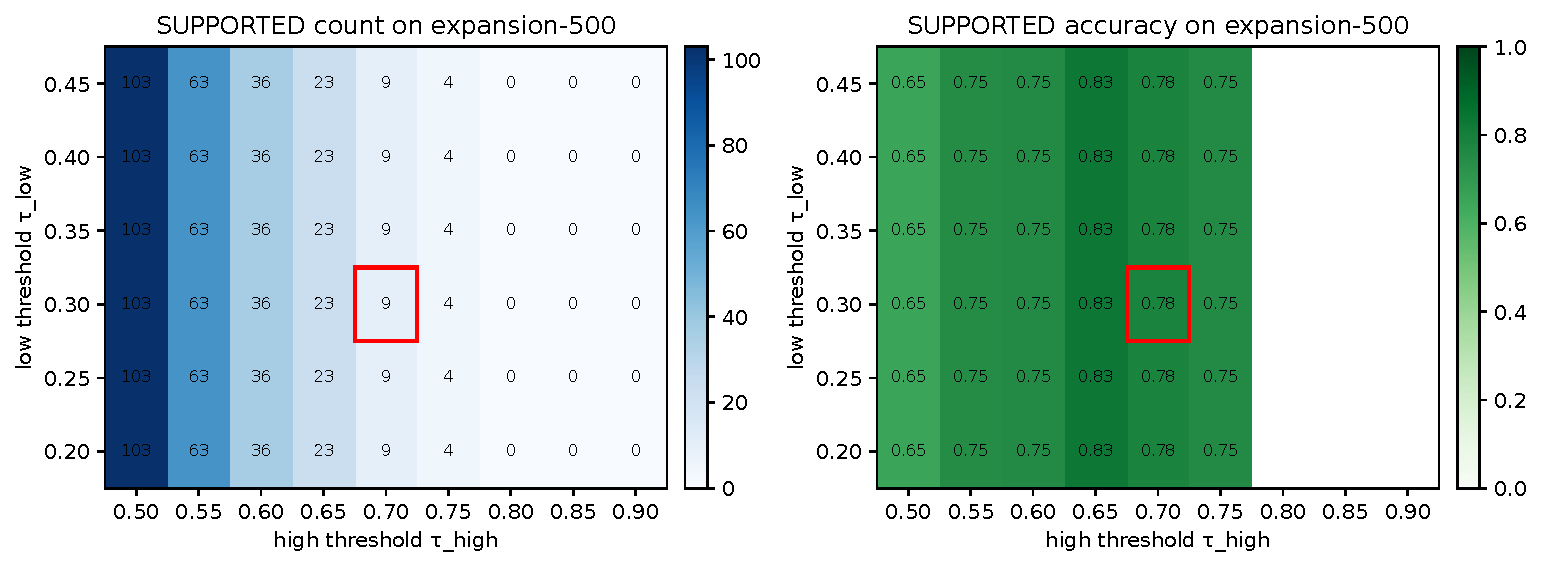
\includegraphics[width=0.98\textwidth]{figures/fig6_threshold_heatmap.pdf}
\caption{Threshold sensitivity. Left: \textsc{Supported} count. Right: \textsc{Supported} accuracy. The paper's default cell $(\SafeNum{0.70}, \SafeNum{0.30})$ is boxed in red.}
\label{fig:threshold-heatmap}
\end{figure}

\end{document}
